\section{مدل سیستم}
\label{sec:system-model}

سامانه چند خوشه نزدیک دارد و هر سرور لبه عضو یک خوشه است. یکی از سرورهای هر خوشه، مدیر آن است و داده سرورهای همان خوشه را دریافت می‌کند. مدیرها گزارش خوشه خود را به ریشه می‌فرستند و تصمیم بین‌خوشه‌ای را از آن دریافت می‌کنند.

کاربر می‌تواند مستقیما به لبه هر خوشه درخواست بدهد. لبه دریافت‌کننده، مبدأ ارسال است و با جدول وزن خود یک نمونه سرویس را انتخاب می‌کند. درخواست کاربر برای ورود به خوشه از ریشه یا خوشه دیگری عبور نمی‌کند.

یک سرور می‌تواند فرستنده درخواست، میزبان سرویس یا هر دو باشد. تقاضا به مبدأ و ظرفیت پردازش به نمونه مقصد مربوط است. مدیر خوشه نیز می‌تواند روی یکی از همین سرورها اجرا شود؛ منابع لازم برای کنترل، پیش از تخصیص پردازنده به کانتینرها کنار گذاشته می‌شوند.

\begin{figure}[H]
\centering
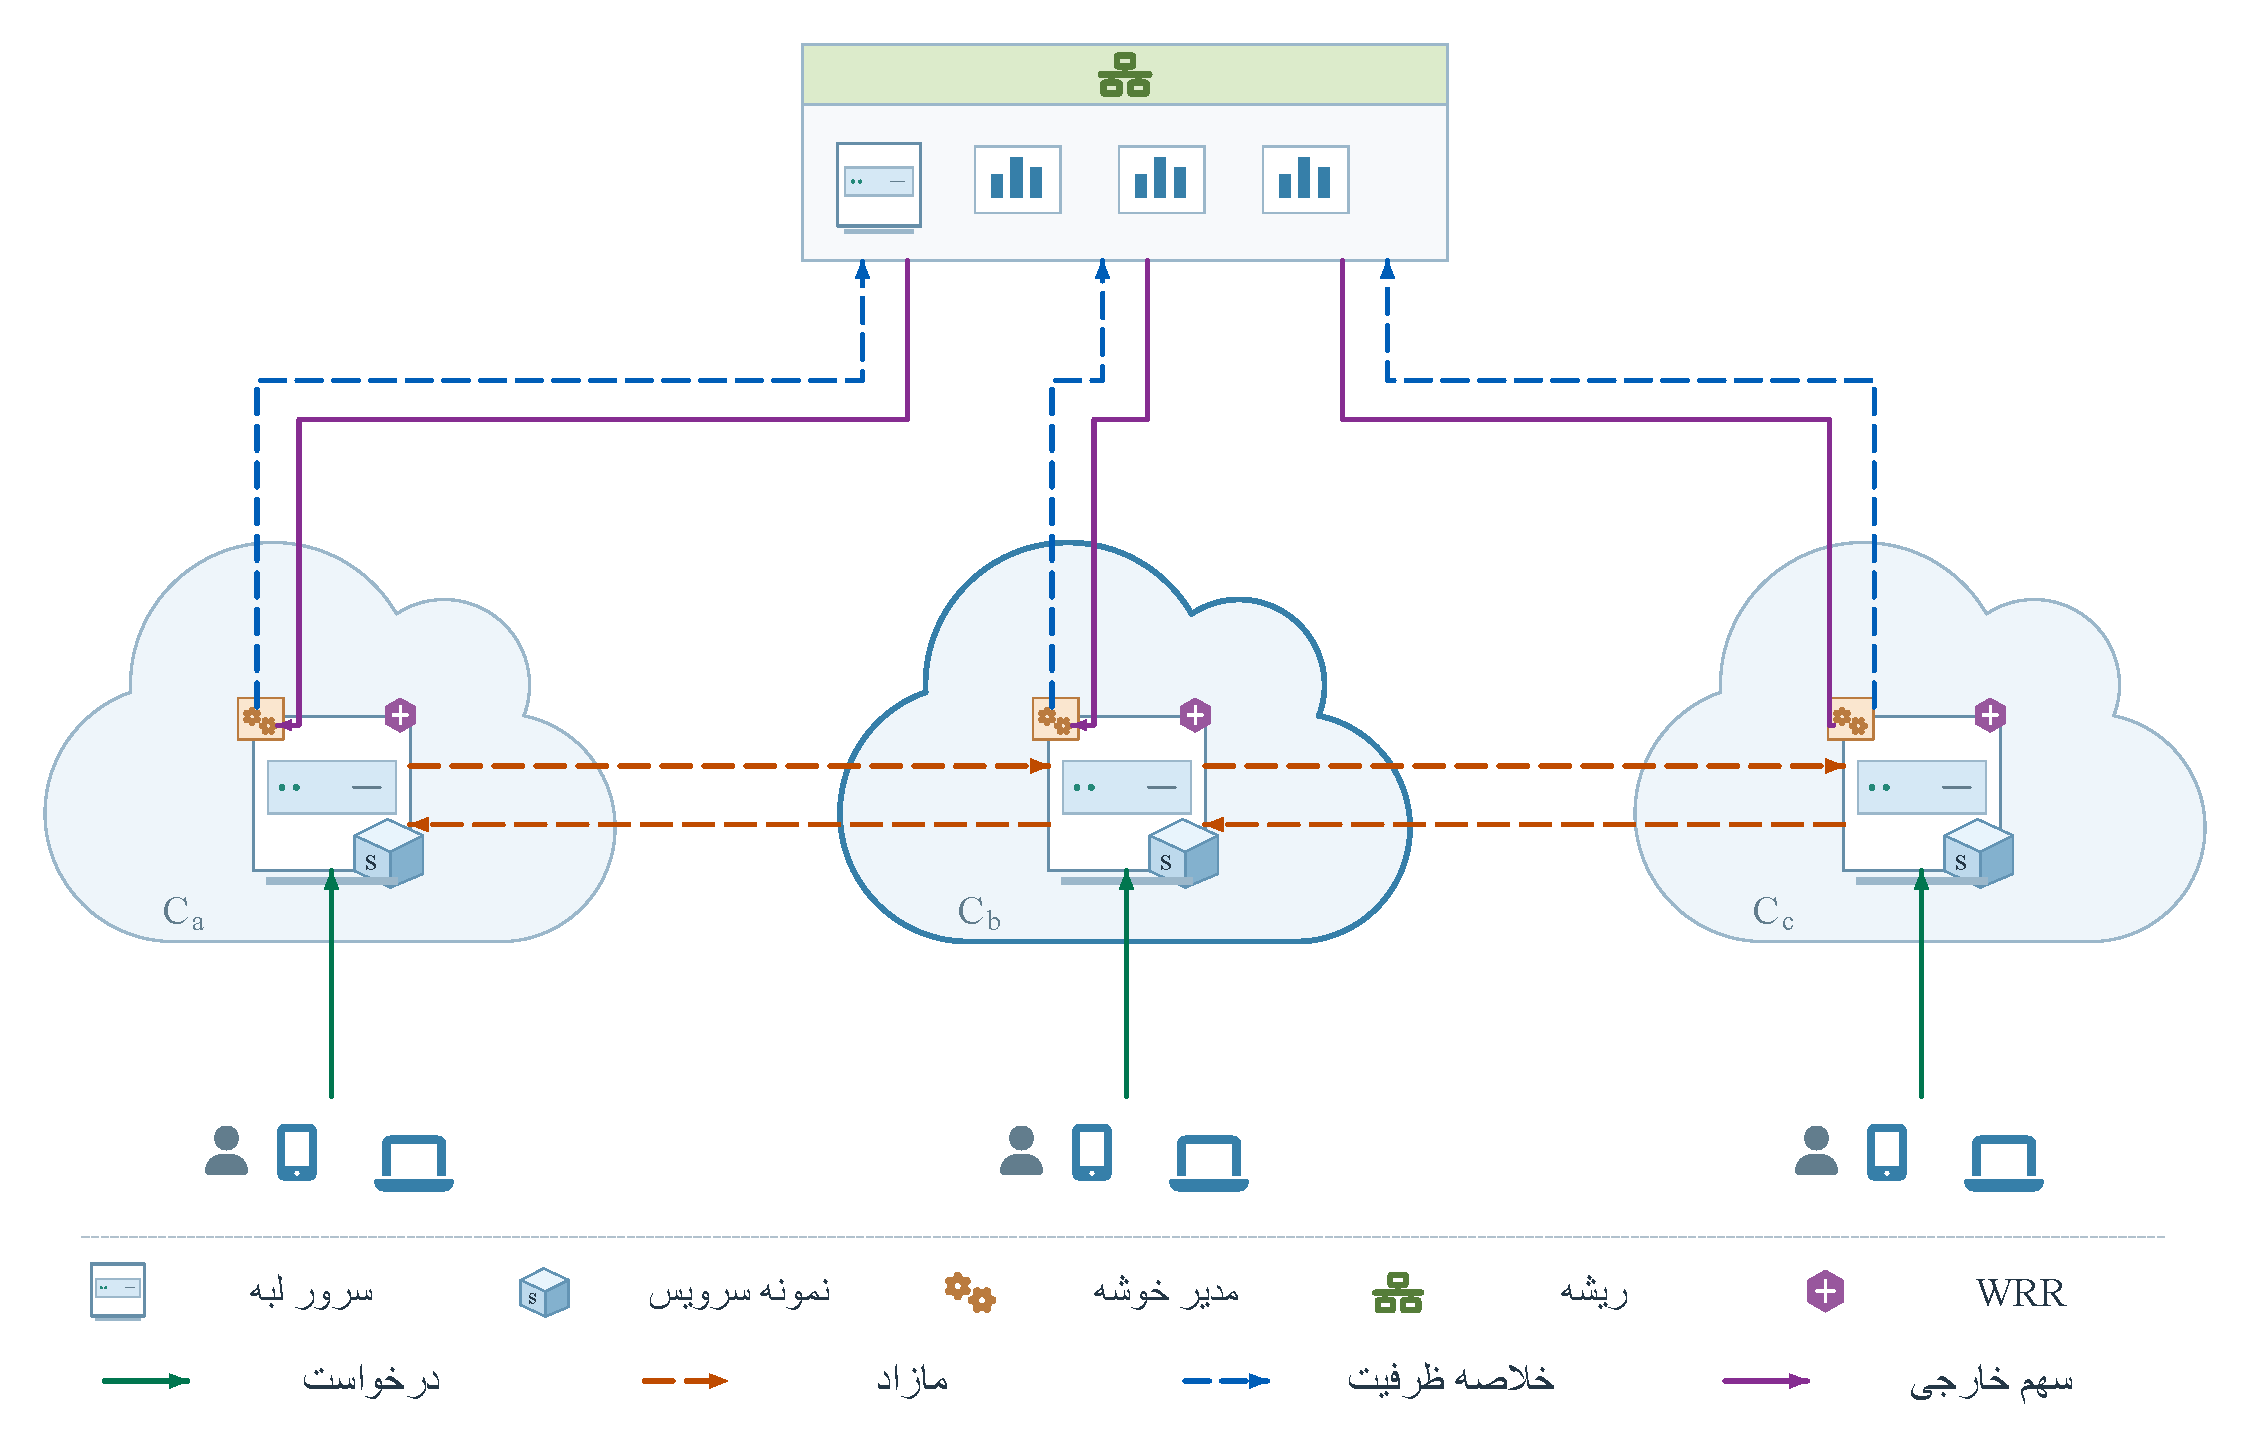
\includegraphics[width=\linewidth]{figures/visio/v10/01-system-model.pdf}
\caption[مدل سیستم و ارتباطات بین خوشه‌ها]{نمای کلی ارتباطات ریشه، خوشه‌ها و کاربران. در هر ابر یک سرور نماینده نشان داده شده است. گزارش ظرفیت به ریشه می‌رود و سهم خارجی به مدیر خوشه برمی‌گردد. پیکان‌های نارنجی بین لبه‌ها، دو زوج مسیر مستقیم ارسال مازاد را نشان می‌دهند. خوشه $C_b$ در شکل~\ref{fig:algorithm-architecture} بزرگ می‌شود.}
\label{fig:system-model}
\end{figure}

در شکل~\ref{fig:system-model}، مسیرهای خارجی برای دو زوج خوشه رسم شده‌اند؛ همین نوع ارتباط مستقیم میان هر زوج مقصد مجاز برقرار می‌شود. خوشه میانی گذرگاه درخواست خوشه‌های دیگر نیست. پیکان‌های گزارش و سهم خارجی فقط مدیرها را به ریشه وصل می‌کنند.

\subsection{اجزا، سرویس‌ها و مرز داده}

در شکل‌ها، $C_a$، $C_b$ و $C_c$ نام خوشه‌ها هستند. در روابط، $a$ و $b$ به‌ترتیب خوشه مبدأ و مقصد، $e$ مبدأ، $s$ سرویس و $i$ نمونه مقصد را نشان می‌دهند. تابع $h(i)$ میزبان فیزیکی نمونه است. هر نمونه در یک کانتینر با سهم مشخص پردازنده اجرا می‌شود و چند کانتینر می‌توانند روی یک میزبان باشند.

در روابط محلی، خوشه از متن معلوم است و شاخص آن برای کوتاه ماندن نمادهایی مانند $\mu_{si}$ تکرار نمی‌شود. در جدول بین‌خوشه‌ای، زوج $(b,i)$ نمونه مقصد را مشخص می‌کند.

اگر نمونه‌های فراخواننده روی یک لبه به سیاست جدا نیاز داشته باشند، شناسه مبدأ $e$ زوج «لبه، نمونه فراخواننده» است؛ روابط بدون افزودن شاخص تازه به کار می‌روند.

مجموعه $\mathcal E_a$ مبدأهای خوشه $a$ است. مجموعه $\mathcal A_{as}$ نمونه‌های سالم، آماده و مجاز سرویس $s$ با برآورد ظرفیت معتبر را نشان می‌دهد. میزبان‌های متمایز همین نمونه‌ها مجموعه $\mathcal H_{as}=\{h(i):i\in\mathcal A_{as}\}$ را می‌سازند؛ فرض می‌شود مبدأهای خوشه به این مجموعه مقصد مشترک دسترسی دارند.

داده خام پردازنده و صف هر سرور فقط در اختیار مدیر همان خوشه است. ریشه شناسه نمونه‌های سرویس و خلاصه ظرفیت آن‌ها را دارد. داده منابع مستقیما بین دو مدیر خوشه ردوبدل نمی‌شود.

مقصدهای خارجی باید از نظر شبکه و مجوز سرویس قابل دسترسی باشند. فهرست نمونه‌های سالم و آماده، ورودی محاسبه وزن است.

\subsection{تقاضا، ظرفیت و بار مشاهده‌شده}

پنجره پایش $\Delta$ قابل تنظیم است و در این متن مقدار پایه آن $5$ ثانیه است. هر تلاش ارسال، مستقل از موفقیت آن، یک بار در مبدأ شمرده می‌شود. اگر بازتلاش فعال باشد، شمار تلاش با شمار درخواست اصلی برنامه جدا نگه داشته می‌شود.

با $A^{\mathrm{src}}_{es}$ آغاز تلاش، نرخ مبدأ و نرخ کل تقاضای همان سرویس در خوشه عبارت‌اند از
\begin{equation}
 D_{es}=\frac{A^{\mathrm{src}}_{es}}{\Delta},\qquad
 D_{as}=\sum_{e\in\mathcal E_a}D_{es}.
 \label{eq:source-demand}
\end{equation}
واحد نرخ، درخواست بر ثانیه است. $D_{as}$ تقاضایی است که توزیع آن از لبه‌های خوشه $a$ آغاز می‌شود؛ درخواست مستقیم کاربران و فراخوانی‌های تولیدشده در این لبه‌ها را در بر می‌گیرد. شمار ورود به کانتینر مقصد، بار دریافتی آن را نشان می‌دهد؛ شمار پردازش‌های پایان‌یافته برای برآورد توان خدمت به کار می‌رود.

ورود درخواست محلی یا خارجی در کانتینر مقصد ثبت می‌شود، اما برای همان درخواست، تقاضای مبدأ دوباره ساخته نمی‌شود. نمونه مقصد درخواست را اجرا می‌کند؛ اگر سرویس دیگری را فراخوانی کند، آن فراخوانی تقاضای تازه همان سرویس است.

هر کانتینر نمونه $i$ از سرویس $s$، سهم قابل اتکای $g_{si}>0$ هسته پردازنده دارد. این سهم می‌تواند کسری از یک هسته باشد. تخصیص‌دهنده منابع باید مجموع سهم کانتینرهای هر میزبان را در هسته‌های قابل استفاده آن جا دهد؛ همین تخصیص، ورودی مدل است.

عامل پایش، مصرف پردازنده کانتینر را در پنجره قبل با $T^{\mathrm{CPU}}_{si}$، بر حسب هسته‌ثانیه، و تعداد پردازش‌های پایان‌یافته را با $N^{\mathrm{proc}}_{si}$ ثبت می‌کند. ظرفیت $\mu_{si}$ از این داده‌ها و سهم هسته، با مدل خطی بخش مدیر خوشه برآورد می‌شود.

ظرفیت هر کانتینر جدا برآورد می‌شود و بار زمینه سرویس‌های دیگر وارد مدل نمی‌شود. اعتبار این ساده‌سازی به تحقق سهم پردازنده و مناسب بودن تقریب خطی وابسته است.

\subsection{مشاهده مسیر، خطا و صف}

مدت هر تلاش با ساعت یکنواخت مبدأ از ارسال تا پاسخ، خطا یا پایان مهلت اندازه‌گیری می‌شود. پینگ، دوره مستقل و قابل تنظیم دارد. پاسخ \lr{API} به زمان پردازش داخلی نیاز ندارد و تفاضل زمان درخواست و پینگ نیز زمان دقیق صف را به دست نمی‌دهد.

برای $n_{ei}>0$ کاوش معتبر، میانگین مسیر چنین است:
\begin{equation}
 \overline d^{\mathrm{net}}_{ei}=\frac{1}{n_{ei}}\sum_{g=1}^{n_{ei}}d_{ei,g}.
 \label{eq:ping-mean}
\end{equation}
نوع کاوش و زمان آخرین مشاهده همراه مقدار نگهداری می‌شوند. نبود کاوش معتبر، پینگ صفر نیست.

اگر $C_{esi}$ پایان موفق و $F_{esi}$ پایان ناموفق باشند، نسبت شکست از همان جمعیت پایان‌ها ساخته می‌شود:
\begin{equation}
 \widehat f_{esi}=\frac{F_{esi}}{C_{esi}+F_{esi}},\qquad C_{esi}+F_{esi}>0.
 \label{eq:failure-observation}
\end{equation}
با $A_k$ آغاز و $O(t_k)$ تلاش در جریان، حسابداری پنجره برابر $O(t_{k+1})=O(t_k)+A_k-C_k-F_k$ است. در مخرج صفر، مشاهده شکست تازه ساخته نمی‌شود؛ مقدار معتبر قبلی و سن آن مشخص می‌مانند. 

در شروع، مقدار اولیه سیاست برای شکست با پرچم «بدون مشاهده» نگه داشته می‌شود. پینگ اولیه مسیر محلی نیز پیش از استفاده در هزینه، با کاوش معتبر به دست می‌آید.

عامل پایش، تعداد منتظران هر کانتینر را از درخواست‌های در حال خدمت جدا ثبت می‌کند. در صورت وجود ابزار، اختلاف زمان ورود به صف و شروع خدمت، انتظار را می‌دهد. زمان \lr{CPU} کل و سهم قابل انتساب سرویس نیز از اختلاف شمارنده‌های پنجره به دست می‌آیند.

مصرف پردازنده نسبت به سهم همان کانتینر نرمال می‌شود: $u_{si}=T^{\mathrm{CPU}}_{si}/(g_{si}\Delta)$. بنابراین، مصرف نیم هسته در کانتینری با سهم یک هسته، $u_{si}=0.5$ است؛ همین مصرف برای سهم دو هسته، $u_{si}=0.25$ است. درصد مصرف کل میزبان جای این نسبت را نمی‌گیرد.

\Needspace{12\baselineskip}
\begin{longtable}{>{\centering\arraybackslash}p{3.3cm}p{9.8cm}}
\caption{نمادهای پایه مدل سیستم}
\label{tab:system-symbols}\\
\toprule نماد & معنی \\ \midrule
$a,b$ & خوشه مبدأ و مقصد \\
$e,s,i,h(i)$ & مبدأ، سرویس، نمونه مقصد و میزبان فیزیکی آن \\
$\mathcal E_a$ & مبدأهای داخل خوشه \\
$\mathcal H_{as},\mathcal A_{as}$ & میزبان‌های متمایز و نمونه‌های مجاز سرویس در خوشه \\
$D_{es},D_{as}$ & تقاضای مبدأ و مجموع تقاضای محلی خوشه برای سرویس \\
$g_{si},T^{\mathrm{CPU}}_{si}$ & سهم هسته کانتینر و زمان مصرف آن در پنجره قبل \\
$N^{\mathrm{proc}}_{si},\mu_{si}$ & شمار پردازش‌های پایان‌یافته و ظرفیت خطی همان کانتینر \\
$\Delta$ & طول پنجره شمارش، ثانیه \\
$\overline d^{\mathrm{net}}_{ei},\widehat f_{esi}$ & میانگین پینگ مسیر و نسبت شکست مشاهده‌شده \\
\bottomrule
\end{longtable}

گزارش هر پنجره، زمان آغاز و پایان، شناسه تولیدکننده، نسخه استقرار و اعتبار مشاهده را دارد. شمارنده تجمعی به اختلاف همان پنجره تبدیل می‌شود و بازنشانی آن تشخیص داده می‌شود. داده خام تک‌درخواست برای ریشه ارسال نمی‌شود.
